\section{Audit and coverage of the records}
\label{sec:audit}

All numbers in this paper come from \NAuditedRecords{} immutable job records written by the campaign (six GPU stratum--engine combinations plus the CPU timing lane), each of which was audited by a program independent of the one that produced it. The audit recomputes every accuracy statistic from the stored arrays and compares it with the stored one, checks the SHA-256 identity of the Python sources, native libraries, helper files, inputs and initial densities against the frozen campaign, verifies that every record's request (case, version, mode, attempt, scientific signature) matches its directory and result, that no timing record carries allocation or profiling instrumentation, that each timing slot is unique, and that every GPU result points to an audited CPU reference. Per stratum the audited record counts are \NRecAHund{} (A100), \NRecVHund{} (V100), \NRecPSixteen{} (P100-16), \NRecPTwelve{} (P100-12), \NRecAHundCupy{} (A100, CuPy engine) and \NRecVHundCupy{} (V100, CuPy engine).

Table~\ref{tab:coverage} and Figure~\ref{fig:status} give the outcome of the memory-mode run of each (case, code version) pair. About 90\% of outcomes on the A100 and V100 are \emph{qualified}: the result reproduces the independent CPU result within the declared gate. The rest are explained in Section~\ref{sec:accuracy}: non-converged cases, accuracy failures (the original code on Taxol, and two job types that fail identically in both code versions) and, on the two P100 cards, genuine memory limits.

\begin{table}[!htbp]
\centering
\small
\resizebox{\textwidth}{!}{%
\begin{tabular}{lrrrrrrr}
\toprule
stratum & outcomes & qualified & accuracy failed & non-converged & resource limited & infrastructure & audited records \\
\midrule
A100 & 248 & 223 & 11 & 14 & 0 & 0 & 2384 \\
V100 & 248 & 224 & 11 & 13 & 0 & 0 & 2399 \\
A100 CuPy & 248 & 222 & 12 & 14 & 0 & 0 & 2247 \\
V100 CuPy & 250 & 224 & 10 & 13 & 0 & 3 & 2265 \\
P100-16 & 248 & 212 & 8 & 14 & 9 & 5 & 2184 \\
P100-12 & 248 & 215 & 8 & 14 & 6 & 5 & 2193 \\
\bottomrule
\end{tabular}}
\caption{Outcomes of the memory-mode run of each (case, code version) pair on each stratum, and the number of audited records. `Infrastructure' on the P100 cards includes plain CUDA out-of-memory errors that the runner labelled generically (see text).}
\label{tab:coverage}
\end{table}

\begin{figure}[!htbp]
\centering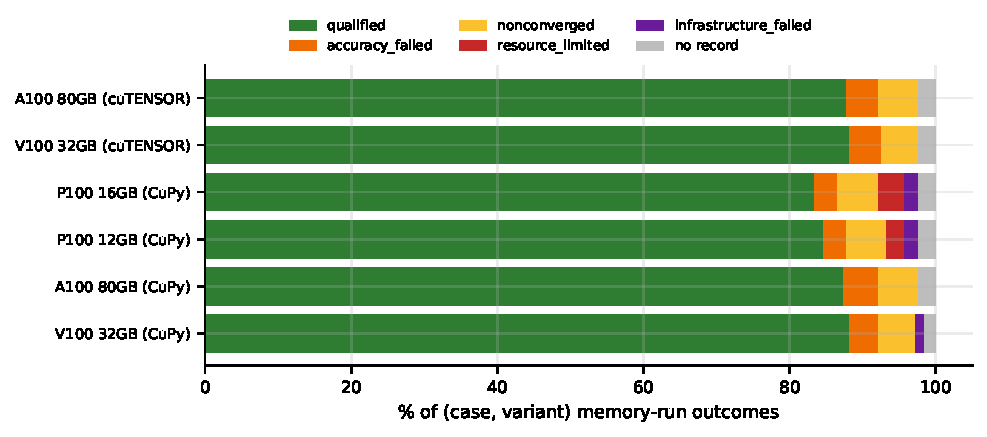
\includegraphics[width=.82\textwidth]{fig_status.pdf}
\caption{Outcome of the memory-mode run of each case and code version on each stratum. ``No record'' are the three open-shell cases (OH with B3LYP, PBE and wB97X) whose CPU reference did not converge and that were not run on the GPU, and the pre-launch rejections noted in Section~\ref{sec:limits}.}
\label{fig:status}
\end{figure}

\section{Accuracy}
\label{sec:accuracy}

\paragraph{Qualified results.} Among all qualified GPU results the largest deviation from CPU PySCF, for both code versions, was $8.6\times10^{-9}$~Eh in the SCF energy (the gate is $10^{-8}$), $9.0\times10^{-7}$~Eh/Bohr in a gradient component (gate $10^{-6}$), $9.6\times10^{-7}$~Eh/Bohr$^2$ in a Hessian element (gate $10^{-5}$), $2.1\times10^{-8}$~Eh in an excitation energy (gate $10^{-6}$), $2.8\times10^{-9}$~Eh in a correlation energy, $2.3\times10^{-7}$~a.u.\ in a polarizability component (gate $10^{-5}$) and $5.3\times10^{-5}$~ppm in a shielding. Figure~\ref{fig:accuracy} shows the distribution. The new code is not less accurate than the original: its worst qualified gradient error ($8.5\times10^{-8}$~Eh/Bohr, for NO with B3LYP on the P100-16) is an order of magnitude below the original's worst ($9.0\times10^{-7}$, tamoxifen B3LYP/def2-TZVP on the V100 with the CuPy engine), and over the 1314 pairs of error values compared the new code's error is smaller in 606, larger in 466 and equal in 242 (median ratio 1.00), so the two versions cannot be distinguished in accuracy at this level; their differences are far below the gates. The worst values lie close to the gates (the gates were set from the numerical noise of the independent CPU reference), so the check demonstrates agreement at the gate level and does not establish a tighter bound.

\begin{figure}[!htbp]
\centering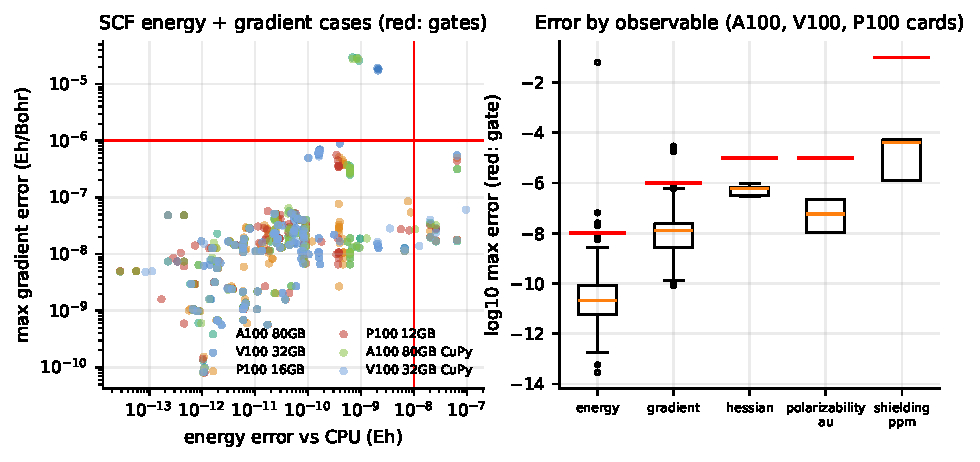
\includegraphics[width=\textwidth]{fig_accuracy.pdf}
\caption{Accuracy against the independent CPU result. Left: SCF energy and maximum gradient error of every energy-plus-gradient case that was run, for both code versions and all strata (red lines: gates; points beyond them are the failures listed in Table~\ref{tab:failures}). Right: log of the maximum error per observable over qualified results (red: gate).}
\label{fig:accuracy}
\end{figure}

\paragraph{Failures.} Table~\ref{tab:failures} lists every group of results that did not qualify. Two of them affect \emph{both} code versions identically on every card, so they are not caused by the changes under test, but are properties of the shared native stack, of the GPU methods or of a setup difference between the codes (not investigated): wB97M-V with its non-local correlation reproduces the CPU energy only to $2$--$6\times10^{-8}$~Eh for benzene, vitamin C and tamoxifen (it passes for H$_2$O at $6.6\times10^{-9}$), and the periodic MgO case differs by $6.4\times10^{-2}$~Eh while periodic silicon agrees to $5\times10^{-10}$~Eh. The wB97M-V offset grows with system size and is identical for the original and new code to the precision recorded; its cause was not investigated here.

\begin{table}[!htbp]
\centering\small
\begin{tabular}{p{4.6cm}p{2.2cm}p{6.7cm}}
\toprule
group & affects & observation \\
\midrule
Taxol HF, B3LYP, wB97X gradients & original only & maximum gradient error about $2\times10^{-5}$~Eh/Bohr against the gate $10^{-6}$; the new code passes (about $5\times10^{-9}$). No equal-accuracy ratio exists for these cases. \\
wB97M-V (benzene, vitamin C, tamoxifen) & both & energy error $2.6\times10^{-8}$, $2.0\times10^{-8}$, $6.4\times10^{-8}$~Eh (gate $10^{-8}$); gradients within the gate. \\
periodic MgO, $\Gamma$ point & both & energy differs by $6.4\times10^{-2}$~Eh on every card. \\
OH (B3LYP, PBE), NO (PBE), OH wB97X probe & all & CPU reference did not converge in 100 cycles from the MINAO guess; excluded. \\
benzene TDA and TDDFT & both & two of five roots flagged non-converged by the GPU solver at the declared tolerance; excitation energies agree with CPU to $1.2\times10^{-9}$~Eh (diagnostic). \\
NO, B3LYP, 48-thread CPU repetitions & CPU lane & two of three repetitions differ from the 24-thread reference by $1.1$ and $1.3\times10^{-8}$~Eh; an ill-conditioned case. \\
CCSD on Pascal (P100) & both & native kernel launch error \texttt{fill\_int4c2e}; cause not diagnosed. \\
Taxol and tamoxifen/TZVP hybrids on P100 & both & GPU memory exhausted (Section~\ref{sec:memory}). \\
\bottomrule
\end{tabular}
\caption{Groups of results that did not qualify. ``Both'' means the original and the new code behave identically.}
\label{tab:failures}
\end{table}

\section{Speed on the datacenter GPUs with cuTENSOR}
\label{sec:speed}

With cuTENSOR installed (the default on the V100 and A100), the new code is \emph{not faster} than the original. Over the 110 cases for which both versions qualified, the median ratio of original to new time is \MedianAllAHund{} on the A100 (range \MinAllAHund--\MaxAllAHund) and \MedianAllVHund{} on the V100 (range \MinAllVHund--\MaxAllVHund); restricting to the \NBigAHund{} (A100) and \NBigVHund{} (V100) cases where the new code takes at least five seconds, so that start-up costs matter less, gives medians of \MedianBigAHund{} and \MedianBigVHund{} (Figure~\ref{fig:violin}). Every job family is within $\pm3\%$ of unity on both cards (Table~\ref{tab:families}): SCF geometric mean 1.00, Hessians 1.00--1.01, TDA/TDDFT 1.00, DF-MP2 and CCSD 0.97--1.01, properties 1.00--1.01, geometry optimizations 1.00--1.01, solvated calculations 0.99--1.00.

\begin{table*}[!htbp]
\centering
\small
\resizebox{\textwidth}{!}{%
\begin{tabular}{lrrrrrrr}
\toprule
family & cases & A100 & V100 & A100 CuPy & V100 CuPy & P100-16 & P100-12 \\
\midrule
correlation & 8 & 0.97 (8) & 1.00 (8) & 1.01 (8) & 1.01 (8) & 1.02 (6) & 0.96 (6) \\
hessian & 8 & 1.00 (8) & 1.01 (8) & 1.03 (8) & 1.02 (8) & 1.02 (8) & 1.02 (8) \\
optimization & 4 & 1.00 (4) & 1.01 (4) & 1.02 (4) & 1.02 (4) & 1.01 (4) & 1.03 (4) \\
pbc & 4 & 0.99 (3) & 1.02 (3) & 1.02 (3) & 1.02 (3) & 1.02 (3) & 1.01 (3) \\
properties & 6 & 1.00 (6) & 1.01 (6) & 1.00 (6) & 1.00 (6) & 1.00 (6) & 0.99 (6) \\
scf & 77 & 1.00 (67) & 1.00 (67) & 1.07 (66) & 1.05 (67) & 1.06 (63) & 1.09 (66) \\
solvent & 8 & 0.99 (8) & 1.00 (8) & 1.05 (8) & 1.05 (8) & 1.07 (8) & 1.14 (8) \\
td & 12 & 1.00 (6) & 1.00 (6) & 1.01 (6) & 1.01 (6) & 1.02 (6) & 1.02 (6) \\
\bottomrule
\end{tabular}}
\caption{Geometric mean of the time ratio original/new per job family (number of cases in brackets); only cases where both versions passed the accuracy gate are included. Values above 1 mean the new code is faster.}
\label{tab:families}
\end{table*}


\begin{figure}[!htbp]
\centering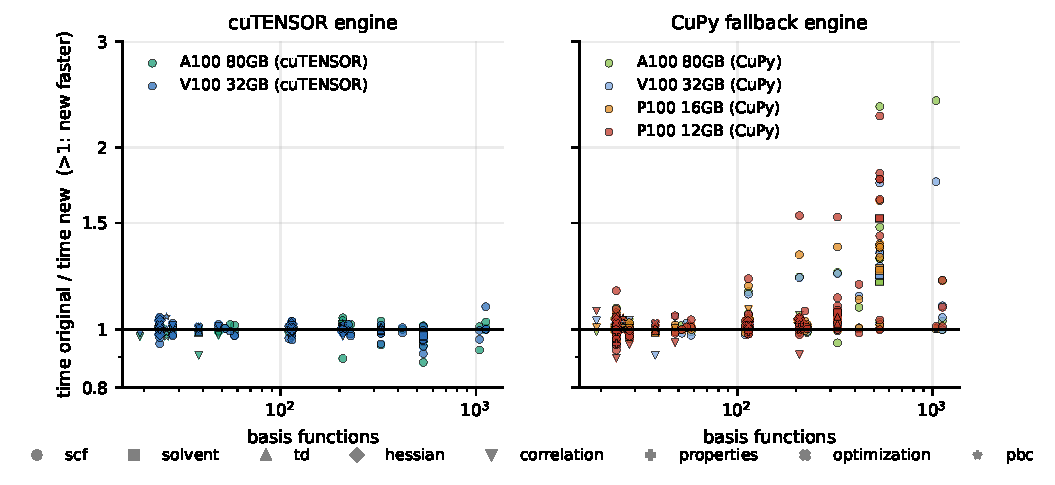
\includegraphics[width=\textwidth]{fig_speed_ratio_vs_size.pdf}
\caption{Time of the original code divided by time of the new code for every case in which both versions qualified, against the number of basis functions (marker shape = job family). Left: cuTENSOR engine. Right: CuPy fallback engine.}
\label{fig:ratio}
\end{figure}

\begin{figure}[!htbp]
\centering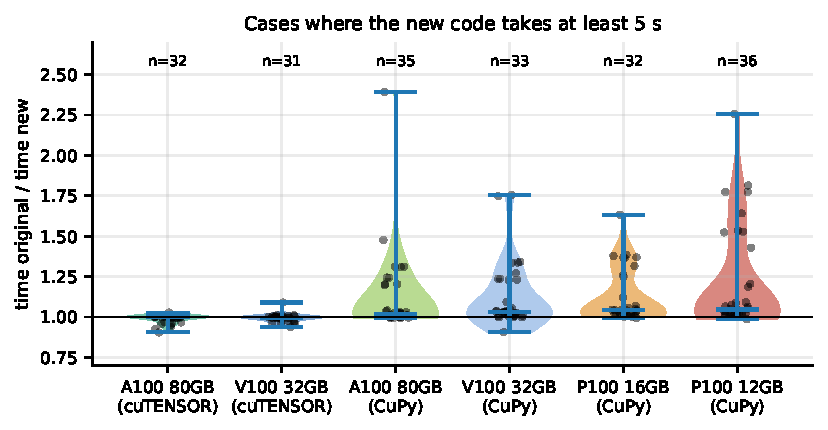
\includegraphics[width=.8\textwidth]{fig_speed_violin.pdf}
\caption{Distribution of the original/new time ratio over cases where the new code takes at least five seconds, per stratum (dots: individual cases).}
\label{fig:violin}
\end{figure}

The larger cases (Table~\ref{tab:large_cutensor}) show where the small differences occur. With the pure functionals LDA, PBE and TPSS the ratios are 0.99--1.09 (Taxol PBE: 1.03 on the A100 and 1.09 on the V100). For hybrid functionals the new code is slightly \emph{slower}: Hartree--Fock tamoxifen 0.88 (A100) and 0.91 (V100) and vitamin C 0.90 (A100), tamoxifen/B3LYP 0.96, tamoxifen/wB97X 0.94, tamoxifen/B3LYP in the larger def2-TZVP basis 0.92 (A100) and 0.96 (V100), and the PCM and SMD solvation cases 0.97. These differences of 3--12\% are small. They recur on both cards, which were measured on shared nodes and are not independent replicates, and they are consistent with the larger gradient cost of the memory-saving gradient (Section~\ref{sec:profile}), although the stage profile does not separate this cost from the other changes.

\begin{table}[!htbp]
\centering
\small
\begin{tabular}{lrrr}
\toprule
case & AOs & A100 & V100 \\
\midrule
\texttt{vitamin\_c-b3lyp-svp} & 208 & 2.34 / 1.04 & 2.18 / 1.01 \\
\texttt{inosine-b3lyp-svp} & 326 & 3.69 / 1.01 & 3.98 / 0.99 \\
\texttt{tamoxifen-lda-svp} & 537 & 4.67 / 1.00 & 4.81 / 0.99 \\
\texttt{tamoxifen-pbe-svp} & 537 & 5.34 / 1.01 & 5.70 / 1.01 \\
\texttt{tamoxifen-tpss-svp} & 537 & 8.05 / 1.01 & 8.72 / 1.00 \\
\texttt{tamoxifen-b3lyp-svp} & 537 & 6.49 / 0.96 & 7.80 / 0.96 \\
\texttt{tamoxifen-wb97x-svp} & 537 & 8.86 / 0.94 & 10.8 / 0.94 \\
\texttt{tamoxifen-pbe-tzvp} & 1042 & 8.48 / 1.01 & 10.8 / 1.00 \\
\texttt{tamoxifen-b3lyp-tzvp} & 1042 & 12.8 / 0.92 & 18.2 / 0.96 \\
\texttt{taxol-lda-svp} & 1123 & 14.5 / 1.01 & 18.3 / 1.00 \\
\texttt{taxol-pbe-svp} & 1123 & 18.0 / 1.03 & 24.2 / 1.09 \\
\texttt{taxol-tpss-svp} & 1123 & 26.4 / 1.00 & 38.1 / 1.00 \\
\texttt{taxol-hf-svp} & 1123 & 25.3 / (G0 acc.) & 47.5 / (G0 acc.) \\
\texttt{taxol-b3lyp-svp} & 1123 & 33.2 / (G0 acc.) & 58.8 / (G0 acc.) \\
\texttt{taxol-wb97x-svp} & 1123 & 49.1 / (G0 acc.) & 85.1 / (G0 acc.) \\
\texttt{tamoxifen-b3lyp-iefpcm} & 537 & 8.57 / 0.97 & 10.4 / 0.97 \\
\texttt{tamoxifen-b3lyp-smd} & 537 & 8.52 / 0.97 & 10.4 / 0.98 \\
\texttt{tamoxifen-wb97mv} & 537 & -- & -- \\
\texttt{vitamin\_c-b3lyp-hessian} & 208 & 20.1 / 1.00 & 20.9 / 0.99 \\
\texttt{inosine-b3lyp-tddft} & 326 & 8.99 / 1.00 & 9.87 / 1.01 \\
\bottomrule
\end{tabular}
\caption{Larger cases, cuTENSOR engine: new-code time in seconds / ratio original-over-new. `mem.' = did not fit in GPU memory or was refused by the memory forecast; `nc' = reference or GPU solver did not converge; `(G0 acc.)' = the original code fails the CPU accuracy gate, so no equal-accuracy ratio exists.}
\label{tab:large_cutensor}
\end{table}


\section{Speed without cuTENSOR: the CuPy fallback and the P100 cards}
\label{sec:engine}

The picture changes when contractions run through the CuPy \texttt{einsum} fallback, which is the only engine on the P100 cards and was forced on the V100 and A100 for a complete second stratum. The new code's Fock-build and gradient contractions use cuBLAS GEMM, GEMV and SYRK directly on this path, whereas the original code calls \texttt{einsum} and pays its repacking and temporaries. Over all cases the median original/new ratio is then \MedianAllAHundCupy{} (A100), \MedianAllVHundCupy{} (V100), \MedianAllPSixteen{} (P100-16) and \MedianAllPTwelve{} (P100-12); over the cases where the new code takes at least five seconds it is \MedianBigAHundCupy{}, \MedianBigVHundCupy{}, \MedianBigPSixteen{} and \MedianBigPTwelve{}, and the SCF family geometric mean is 1.05--1.09 (Table~\ref{tab:families}). The gain is largest in hybrid-functional cases of intermediate size (Table~\ref{tab:large_cupy}): tamoxifen with B3LYP 1.31 (A100) to 1.77 (P100-12), with wB97X 1.27--1.64, with PCM or SMD 1.20--1.53, and tamoxifen/B3LYP in def2-TZVP \MaxAllAHundCupy{} on the A100 and 1.76 on the V100; the GGA functionals gain little (PBE 1.00--1.04), whereas the meta-GGA TPSS, which has no exchange build, gains 1.24--1.43 for tamoxifen and 1.05--1.21 for Taxol (not investigated). The largest ratio observed in any stratum is \MaxAllAHundCupy{} (A100, CuPy engine).

\begin{table}[!htbp]
\centering
\small
\resizebox{\textwidth}{!}{%
\begin{tabular}{lrrrrr}
\toprule
case & AOs & A100 CuPy & V100 CuPy & P100-16 & P100-12 \\
\midrule
\texttt{vitamin\_c-b3lyp-svp} & 208 & 2.27 / 1.03 & 2.30 / 1.02 & 3.21 / 1.02 & 3.49 / 1.03 \\
\texttt{inosine-b3lyp-svp} & 326 & 4.00 / 1.02 & 4.39 / 1.05 & 6.55 / 1.05 & 7.01 / 1.09 \\
\texttt{tamoxifen-lda-svp} & 537 & 4.70 / 1.01 & 4.75 / 1.00 & 7.28 / 1.00 & 7.61 / 1.00 \\
\texttt{tamoxifen-pbe-svp} & 537 & 5.43 / 1.03 & 5.71 / 1.02 & 8.75 / 1.02 & 9.46 / 1.04 \\
\texttt{tamoxifen-tpss-svp} & 537 & 9.04 / 1.24 & 9.00 / 1.24 & 13.7 / 1.36 & 14.2 / 1.43 \\
\texttt{tamoxifen-b3lyp-svp} & 537 & 6.67 / 1.31 & 8.64 / 1.34 & 12.0 / 1.39 & 13.4 / 1.77 \\
\texttt{tamoxifen-wb97x-svp} & 537 & 9.20 / 1.48 & 12.2 / 1.27 & 16.8 / 1.32 & 19.2 / 1.64 \\
\texttt{tamoxifen-pbe-tzvp} & 1042 & 8.55 / 1.00 & 10.9 / 1.00 & 17.7 / 1.01 & 20.4 / 1.01 \\
\texttt{tamoxifen-b3lyp-tzvp} & 1042 & 12.7 / 2.39 & 18.5 / 1.76 & -- & -- \\
\texttt{taxol-lda-svp} & 1123 & 14.6 / 1.00 & 18.5 / 1.00 & -- & 34.5 / 1.01 \\
\texttt{taxol-pbe-svp} & 1123 & 17.9 / 1.03 & 24.3 / 1.09 & -- & 46.1 / 1.09 \\
\texttt{taxol-tpss-svp} & 1123 & 27.6 / 1.20 & 39.3 / 1.05 & -- & 69.8 / 1.21 \\
\texttt{taxol-hf-svp} & 1123 & 24.6 / (G0 acc.) & -- & mem. & mem. \\
\texttt{taxol-b3lyp-svp} & 1123 & 32.8 / (G0 acc.) & -- & mem. & mem. \\
\texttt{taxol-wb97x-svp} & 1123 & 48.5 / (G0 acc.) & -- & mem. & mem. \\
\texttt{tamoxifen-b3lyp-iefpcm} & 537 & 8.83 / 1.20 & 11.4 / 1.23 & 16.1 / 1.26 & 18.0 / 1.52 \\
\texttt{tamoxifen-b3lyp-smd} & 537 & 8.69 / 1.20 & 11.2 / 1.23 & 16.0 / 1.25 & 18.0 / 1.53 \\
\texttt{tamoxifen-wb97mv} & 537 & -- & -- & -- & -- \\
\texttt{vitamin\_c-b3lyp-hessian} & 208 & 26.1 / 1.04 & 25.3 / 1.04 & 37.8 / 1.04 & 36.3 / 1.04 \\
\texttt{inosine-b3lyp-tddft} & 326 & 10.2 / 1.01 & 11.6 / 1.03 & 17.1 / 1.07 & 21.4 / 1.05 \\
\bottomrule
\end{tabular}}
\caption{Larger cases, CuPy fallback engine: new-code time in seconds / ratio original-over-new. `mem.' = did not fit in GPU memory or was refused by the memory forecast; `nc' = reference or GPU solver did not converge; `(G0 acc.)' = the original code fails the CPU accuracy gate, so no equal-accuracy ratio exists.}
\label{tab:large_cupy}
\end{table}


Figure~\ref{fig:engine} shows why. It comes from separate, instrumented profile runs with synchronized stage timers, whose absolute times are about 2\,s above those of the main matrix (Table~\ref{tab:large_cutensor}) and are comparable only with one another. In these runs, for tamoxifen with B3LYP the original code takes 8.3 s with cuTENSOR on the A100 and 10.4 s with the CuPy engine (7.9 and 14.3 s on the V100), while the new code takes 8.7 and 8.8 s on the A100 (8.3 and 9.2 s on the V100): the new code makes the fallback engine as fast as cuTENSOR, but with cuTENSOR installed its fast paths are bypassed and it gains nothing. Put differently, the changes remove a penalty that only the fallback engine pays. This is the regime of the earlier GB10 study (Appendix~\ref{sec:gb10}), where speed-ups of 1.47 (tamoxifen) and 1.95 (Taxol) were measured without cuTENSOR; the cluster data reproduce the direction and show that it depends on the engine, but with smaller factors (1.2--1.8 for tamoxifen hybrids); the GB10 tamoxifen factor (1.47) lies within this range, and its Taxol factor (1.95) is not an equal-accuracy comparison.

\begin{figure}[!htbp]
\centering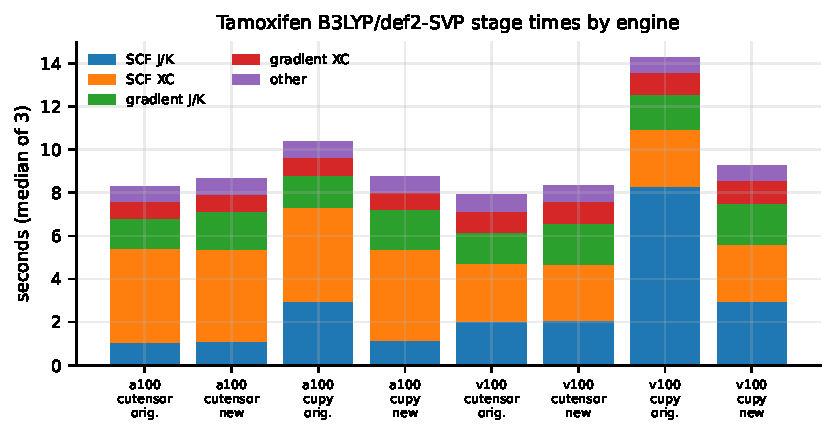
\includegraphics[width=.85\textwidth]{fig_engine_profile.pdf}
\caption{Stage times of tamoxifen B3LYP/def2-SVP (median of three, synchronized timers) for the original and new code with each engine. With cuTENSOR both versions take about 8--9 s; with the CuPy fallback the original code is slower (10.4 s on the A100, 14.3 s on the V100) and the new code is unchanged.}
\label{fig:engine}
\end{figure}

\section{Where the time goes and what did not help}
\label{sec:profile}

\paragraph{Stage profile.} Figure~\ref{fig:taxol} splits the Taxol B3LYP/def2-SVP workflow (20 SCF cycles) into stages. On the A100 the SCF takes 21.9 s (new code), of which the Fock build is 13.9 s (including 3.5 s to build the fitted integrals once), the XC quadrature 7.1 s and the diagonalization 0.4 s; the gradient takes 13.0 s, 76\% of it in the DF Coulomb and exchange derivatives. On the V100 the Fock build dominates even more (32.7 of 42.2 s SCF), as expected from its lower double-precision rate. The grid itself is built in about 0.1 s.

\begin{figure}[!htbp]
\centering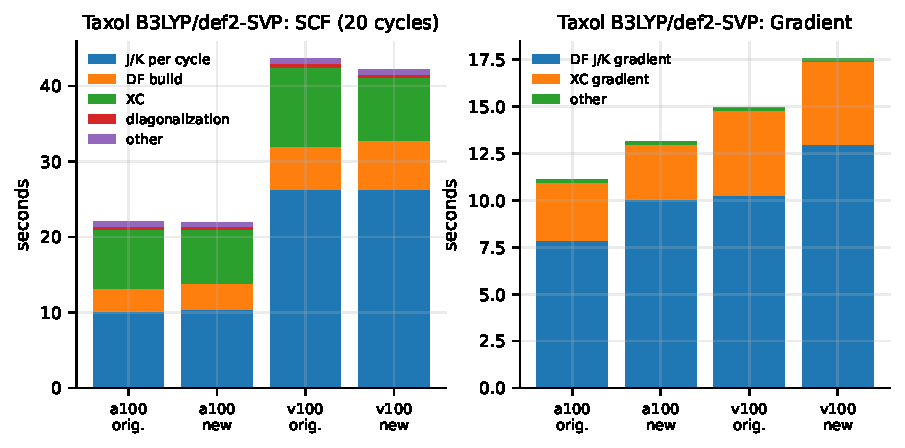
\includegraphics[width=\textwidth]{fig_taxol_stages.pdf}
\caption{Stage times of Taxol B3LYP/def2-SVP on the A100 and V100 with cuTENSOR, original (orig.) and new code. The new code's gradient is 2--3 s slower, the price of its much smaller gradient memory.}
\label{fig:taxol}
\end{figure}

\paragraph{The matrix products are near the measured cuBLAS rate.} A micro-benchmark of the exchange-build contractions at the real Taxol shapes (Figure~\ref{fig:gemm}) shows both the cuTENSOR path and the cuBLAS GEMM/SYRK path running at 14--15 TFLOPS on the A100 (the measured cuBLAS ceiling is 16.3) and 5.8 TFLOPS on the V100 (ceiling 6.8), i.e.\ 85--92\% of the measured cuBLAS rate for the best block sizes (a single block is timed and scaled to the full auxiliary basis, so these are not in-workflow rates); the GEMM/SYRK path is 0--13\% faster per cycle. There is little left to gain from tuning these products.

\begin{figure}[!htbp]
\centering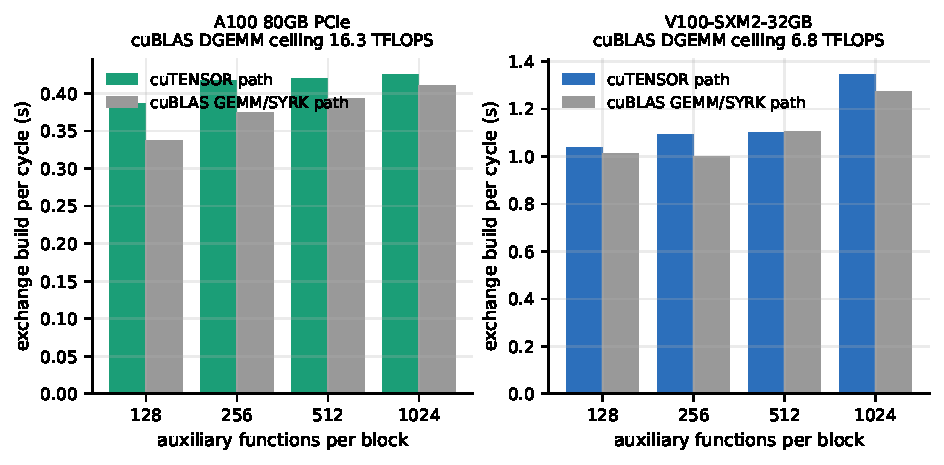
\includegraphics[width=.95\textwidth]{fig_gemm.pdf}
\caption{Estimated exchange-build time per SCF cycle for Taxol (one block of auxiliary functions timed, scaled to the full auxiliary basis) for the cuTENSOR contraction and the cuBLAS GEMM/SYRK path.}
\label{fig:gemm}
\end{figure}

\paragraph{Experiments that did not pay.}
\begin{itemize}[leftmargin=*,itemsep=1pt]
\item \emph{Gradient workspace cap.} Sweeping the fixed workspace budget of the new gradient (1, 2, 4, 8, 16\,GiB and unlimited) changed the Taxol gradient time by less than 1\% above 2\,GiB (13.0--13.1 s on the A100, 17.5--17.6 s on the V100), and by 8\% at 1\,GiB. The planner already chooses the same batch size at the default.
\item \emph{SCF cycle count.} Table~\ref{tab:cycles} and Figure~\ref{fig:cycles}: other starting guesses are equal (atomic densities) or much worse (H\"uckel, VSAP); a DIIS space of 12 saves one or two cycles; a two-stage scheme (coarse grid first) reduces the full-quality cycles from 20 to 12 for Taxol but its cheap pre-cycles cost as much (22.0 s against 22.2 s). Second-order SCF failed in all runs with a CuPy-to-NumPy conversion error.
\item \emph{Cached staging buffers for the disk tier} (a code-review suggestion): an alternating A/B/A/B comparison gave 265, 239~s (without) against 254, 280~s (with); the run-to-run spread exceeds any difference and the change was reverted.
\end{itemize}

\begin{table}[!htbp]
\centering
\small
\begin{tabular}{lrrr}
\toprule
strategy & vitamin C & tamoxifen & Taxol \\
\midrule
MINAO (baseline) & 18 / 3.8 & 18 / 6.0 & 20 / 22.2 \\
superposition of atomic densities & 18 / 4.0 & 19 / 6.0 & 21 / 22.5 \\
extended H\"uckel & 24 / 3.9 & 28 / 7.3 & 39 / 36.7 \\
superposition of atomic potentials & 23 / 5.7 & 27 / 24.7 & 39 / 153.2 \\
MINAO, DIIS space 12 & 16 / 3.5 & 17 / 5.7 & 19 / 21.6 \\
two-stage (coarse grid first) & 11 / 3.5 & 12 / 5.6 & 12 / 22.0 \\
second-order (SOSCF) & failed & failed & failed \\
\bottomrule
\end{tabular}
\caption{SCF cycles at full quality / total SCF seconds on the A100 for different starting guesses and convergence strategies (all reach the same energy within $10^{-8}$ Eh).}
\label{tab:cycles}
\end{table}

\begin{figure}[!htbp]
\centering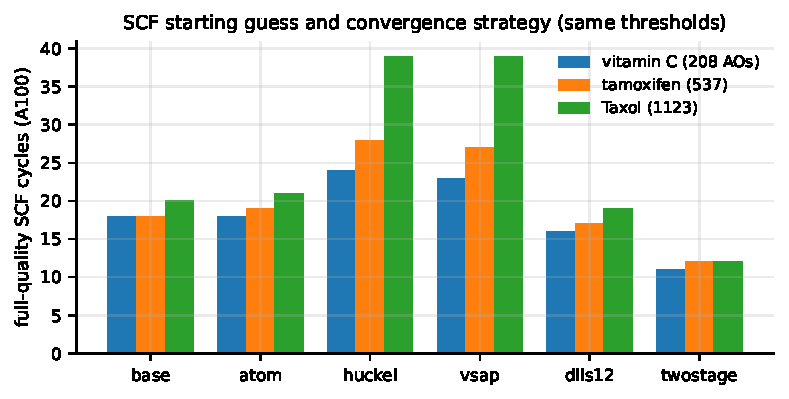
\includegraphics[width=.75\textwidth]{fig_scf_cycles.pdf}
\caption{SCF cycles at full quality for different starting guesses and convergence strategies on the A100.}
\label{fig:cycles}
\end{figure}

\section{First-process (cold start) cost}
\label{sec:cold}

CuPy compiles some kernels at run time. The first process on a node with an empty kernel cache therefore takes much longer than a repeat (Table~\ref{tab:cold} and Figure~\ref{fig:cold}): the H$_2$O B3LYP workflow takes 12.6--23.0 s the first time and 0.9--1.9 s with a populated cache, an overhead of 11--22 s that is similar for the original and the new code and is largest on the 12\,GB P100. The principal timings of this paper use a persistent cache; the figure matters mainly for short jobs and for users whose cache is not preserved between runs.

\begin{table}[!htbp]
\centering
\small
\resizebox{\textwidth}{!}{%
\begin{tabular}{lllrrrrr}
\toprule
card & engine & code & H$_2$O cold (s) & H$_2$O warm (s) & tamoxifen cold (s) & tamoxifen warm (s) & first-process overhead (s) \\
\midrule
A100 & cupy & original & 17.6 & 1.90 & 11.3 & 10.8 & 15.7 \\
 & cupy & new & 19.2 & 1.84 & 8.67 & 8.58 & 17.3 \\
 & cutensor & original & 19.6 & 1.94 & 8.36 & 8.14 & 17.7 \\
 & cutensor & new & 17.5 & 1.81 & 8.37 & 8.55 & 15.7 \\
V100 & cupy & original & 14.5 & 1.03 & 12.2 & 11.6 & 13.5 \\
 & cupy & new & 13.4 & 0.91 & 9.19 & 8.47 & 12.5 \\
 & cutensor & original & 13.0 & 0.86 & 7.56 & 7.37 & 12.2 \\
 & cutensor & new & 12.6 & 0.89 & 7.63 & 7.59 & 11.7 \\
P100-16 & cupy & original & 17.8 & 1.21 & 17.2 & 16.7 & 16.6 \\
 & cupy & new & 17.6 & 1.20 & 12.0 & 12.1 & 16.4 \\
P100-12 & cupy & original & 23.0 & 1.35 & 28.3 & 25.5 & 21.7 \\
 & cupy & new & 22.4 & 1.32 & 14.2 & 14.2 & 21.1 \\
\bottomrule
\end{tabular}}
\caption{Cold start: the first process with an empty CuPy kernel cache against a repeat with the cache populated (workflow time inside the process, imports excluded). Only the first process of each pass is truly cold, so the first-process overhead is the H$_2$O cold time minus its warm time; the later, larger cases of the cold pass reuse kernels compiled by H$_2$O.}
\label{tab:cold}
\end{table}

\begin{figure}[!htbp]
\centering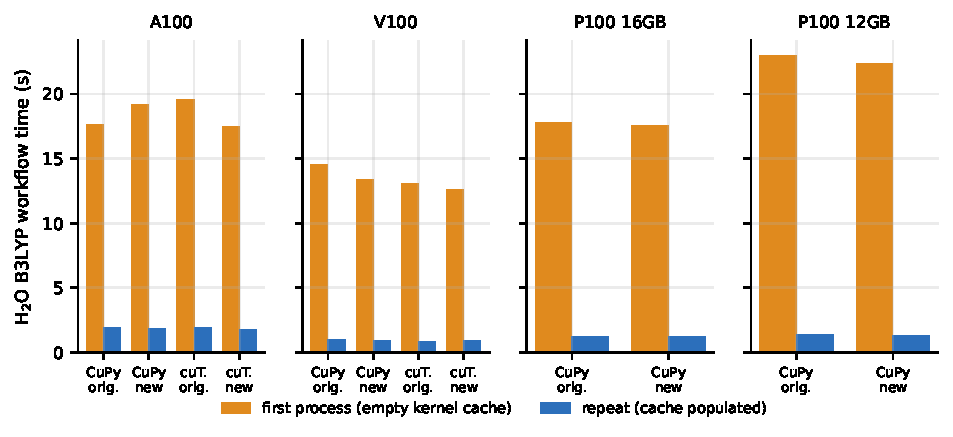
\includegraphics[width=\textwidth]{fig_cold_start.pdf}
\caption{H$_2$O B3LYP/def2-SVP workflow time in the first process after the kernel cache was emptied and in a repeat.}
\label{fig:cold}
\end{figure}

\section{CPU baseline and the GPU speed-up over the CPU}
\label{sec:cpu}

The study optimizes the GPU code, so the CPU is required only to be a fair baseline. The first CPU timing lane used a whole 48-core node with 48 OpenMP and BLAS threads, as the default whole-node setting. For mid-size systems this turned out to be a poor configuration: tamoxifen B3LYP/def2-SVP took 1663 s with 48 threads and default BLAS but 358 s with 24 threads in the scan (a single earlier 24-thread reference run, taken for the accuracy comparison and not as a timing measurement, took 519 s), with identical SCF iterations and energies. Over the complete 24-thread lane the same pattern holds: the 24-thread, one-BLAS-thread run was the faster lane in 120 of the 123 cases with both lanes; for the 65 cases that take at least 20\,s on 48 threads it is faster by a median of 2.0$\times$, and by up to 33$\times$ for the finite-difference benzene HF Hessian (4614 s against 141 s). A thread scan on the five representative cases (Table~\ref{tab:cpuscan}, Figure~\ref{fig:cpuscan}) found the cause: with 48 OpenMP threads each thread's BLAS calls spawn 48 more, oversubscribing the node. Setting BLAS threads to one restores the performance (tamoxifen 364 s at 48 threads, 307 s at 24 threads; vitamin C 24 s and 21 s against 55 s), pinning helps little, and for small molecules fewer threads are better still: benzene is fastest with 12 threads (4.0 s against 17.7 s with 48); H$_2$O is the exception, fastest with 48 threads (3.5 s), and for it and benzene the scan has no one-BLAS-thread runs. For Taxol with PBE the spread is 24\% (1594--1972 s). A second lane with 24 threads and one BLAS thread was therefore run for every case, and the fair CPU baseline of each case is the faster of the two lanes.

\begin{table*}[!htbp]
\centering
\small
\resizebox{\textwidth}{!}{%
\begin{tabular}{lrrrrrrrrrrr}
\toprule
case & 1 & 2 & 4 & 8 & 12 & 24 & 48 & 24/B1 & 48/B1 & 24 pin & 48 pin \\
\midrule
H$_2$O & 4.54 & 4.30 & 4.13 & 4.12 & 4.11 & 4.58 & \textbf{3.52} & -- & -- & -- & -- \\
benzene & 15.3 & 9.06 & 6.07 & 4.33 & \textbf{4.01} & 7.80 & 17.7 & -- & -- & -- & -- \\
vitamin C & -- & -- & -- & -- & 22.3 & 23.5 & 55.3 & \textbf{20.6} & 24.0 & 23.5 & 43.2 \\
tamoxifen & -- & -- & -- & -- & 319.8 & 357.8 & 1663 & \textbf{307.1} & 363.8 & 322.2 & 946.6 \\
Taxol PBE & -- & -- & -- & -- & 1972 & 1604 & 1717 & \textbf{1594} & 1622 & 1604 & 1700 \\
\bottomrule
\end{tabular}}
\caption{CPU thread scan, wall time in seconds on one 48-core node. Columns: OpenMP threads with BLAS threads equal to OpenMP threads; `B1' = BLAS threads set to 1; `pin' = OpenMP threads pinned to cores. Bold: fastest for that case.}
\label{tab:cpuscan}
\end{table*}

\begin{figure}[!htbp]
\centering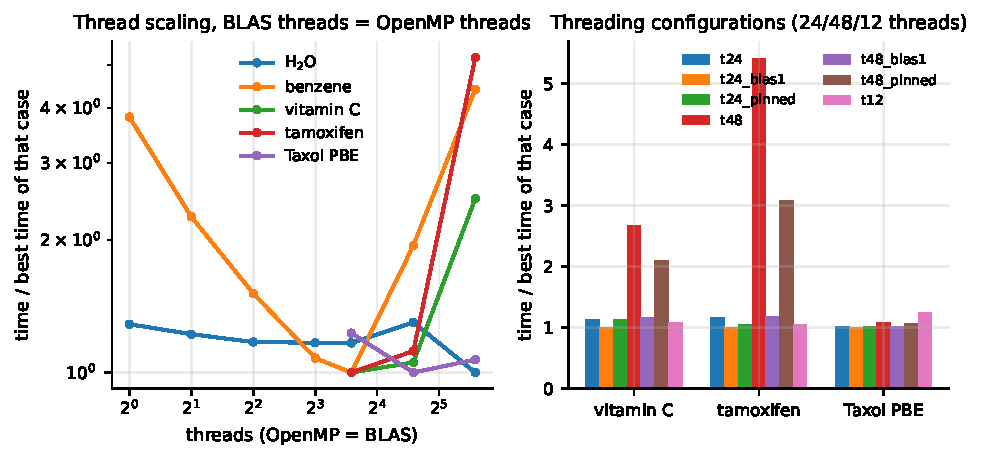
\includegraphics[width=\textwidth]{fig_cpu_scan.pdf}
\caption{CPU thread scaling. Left: time relative to the best configuration against thread count (BLAS threads equal to OpenMP threads). Right: threading configurations for the three larger cases.}
\label{fig:cpuscan}
\end{figure}

Table~\ref{tab:cpugpu} and Figure~\ref{fig:cpugpu} compare the CPU with the new GPU code. For the cases in which the CPU needs at least 20 s (\CPUNBestAHund{} on the A100, \CPUNBestVHund{} on the V100, \CPUNBestPSixteen{} on the P100-16) the median speed-up of the A100, V100 and P100-16 is \CPUMedBestAHund, \CPUMedBestVHund{} and \CPUMedBestPSixteen{} against the best CPU lane, with maxima of \CPUMaxBestAHund, \CPUMaxBestVHund{} and \CPUMaxBestPSixteen; the largest ratios belong to the finite-difference Hessians, which the CPU computes from many gradients. For small jobs the GPU gains little: it is slower than the best CPU lane in 39 of 113 cases on the A100 (36 and 38 on the V100 and P100-16) and less than three times faster in 56 A100 cases, among them (H$_2$O with HF, direct SCF, DF-MP2, CCSD, polarizability and shielding, and the formaldehyde wB97X TDA) with CPU times of a few seconds or less, where GPU start-up and small kernels dominate. The CPU baseline columns of the table state which lane was used.

\CPULaneNote

\begin{table*}[!htbp]
\centering
\small
\resizebox{\textwidth}{!}{%
\begin{tabular}{lrrrrrrr}
\toprule
case & AOs & CPU 48 thr (s) & CPU best (s) & A100 new (s) & V100 new (s) & P100-16 new (s) & speed-up A100 \\
\midrule
\texttt{h2o-b3lyp-svp} & 24 & 3.16 & 0.51 (cpu24b1) & 1.01 & 0.99 & 1.22 & 1 \\
\texttt{benzene-b3lyp-svp} & 114 & 17.7 & 3.67 (cpu24b1) & 1.28 & 1.31 & 1.69 & 3 \\
\texttt{vitamin\_c-b3lyp-svp} & 208 & 51.7 & 17.3 (cpu24b1) & 2.34 & 2.18 & 3.21 & 7 \\
\texttt{inosine-b3lyp-svp} & 326 & 118.8 & 72.4 (cpu24b1) & 3.69 & 3.98 & 6.55 & 20 \\
\texttt{tamoxifen-b3lyp-svp} & 537 & 1654 & 310.6 (cpu24b1) & 6.49 & 7.80 & 12.0 & 48 \\
\texttt{tamoxifen-b3lyp-tzvp} & 1042 & 683.0 & 593.6 (cpu24b1) & 12.8 & 18.2 & 26.0 & 46 \\
\texttt{taxol-pbe-svp} & 1123 & 1702 & 1604 (cpu24b1) & 18.0 & 24.2 & 39.3 & 89 \\
\texttt{taxol-tpss-svp} & 1123 & 2504 & 2063 (cpu24b1) & 26.4 & 38.1 & 60.6 & 78 \\
\texttt{vitamin\_c-b3lyp-hessian} & 208 & 20730 & 5268 (cpu24b1) & 20.1 & 20.9 & 37.8 & 262 \\
\texttt{inosine-b3lyp-tddft} & 326 & 949.1 & 790.2 (cpu24b1) & 8.99 & 9.87 & 17.1 & 88 \\
\texttt{tamoxifen-b3lyp-iefpcm} & 537 & 1931 & 927.4 (cpu24b1) & 8.57 & 10.4 & 16.1 & 108 \\
\texttt{vitamin\_c-dfmp2} & 208 & 18.7 & 2.13 (cpu24b1) & 1.11 & 1.17 & 1.59 & 2 \\
\bottomrule
\end{tabular}}
\caption{CPU wall time against the new GPU code. CPU 48 thr: whole 48-core node, default settings; CPU best: the faster of the available CPU lanes (configuration in brackets); speed-up = CPU best / A100.}
\label{tab:cpugpu}
\end{table*}

\begin{figure}[!htbp]
\centering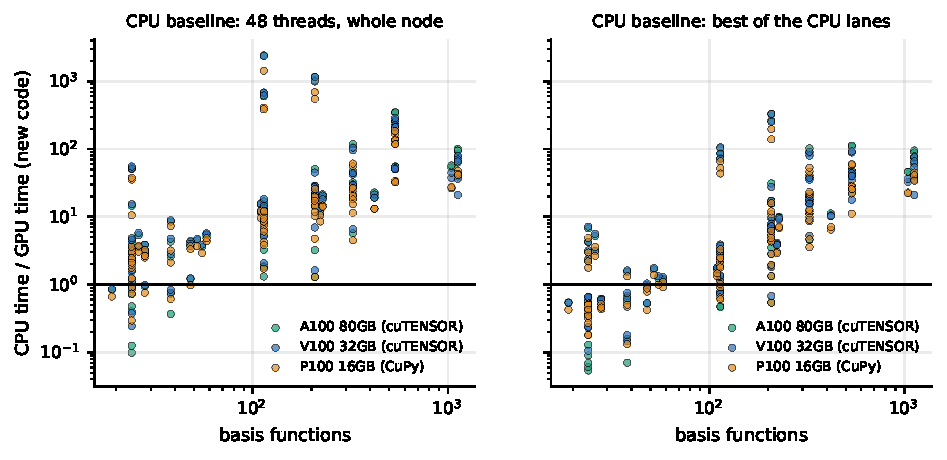
\includegraphics[width=\textwidth]{fig_cpu_vs_gpu.pdf}
\caption{CPU time divided by new-GPU time against system size. Left: CPU baseline from the 48-thread whole-node lane only. Right: baseline from the faster of the available CPU lanes.}
\label{fig:cpugpu}
\end{figure}

\section{Memory and capacity}
\label{sec:memory}

\subsection{GPU memory of the workflow}

The new code needs less GPU memory for every case that contains an exchange build and a gradient (Figure~\ref{fig:memory} and Table~\ref{tab:memory}). Over the \MemN{} cases with an original peak above 0.3~GB on the V100 the median reduction is \MemMedian$\times$ (range \MemMin--\MemMax$\times$): tamoxifen B3LYP falls from 15.9 to 4.4~GB (3.7$\times$), PCM and SMD cases 2.9--3.7$\times$, tamoxifen in def2-TZVP from 24.3 to 11.6~GB (2.1$\times$), and Taxol with the pure functionals LDA, PBE and TPSS 3.5--4.8$\times$ (from about 5 to 1--1.5~GB). Taxol with the hybrid functionals falls from 29.5 to 20.0~GB (HF, B3LYP; 1.5$\times$) and, for wB97X, from 29.6 to 25.9~GB (1.1$\times$). Hessians, TDA/TDDFT and DF-MP2 are unchanged (1.00$\times$): the changes do not touch their code paths, so the median above includes jobs that are not affected (over the 41 V100 cases with a reduction above 5\% it is 2.7$\times$). The figures depend on the stratum, because the original code sizes its gradient workspace from the free memory of the card: the medians are 1.8--2.5$\times$ over the six strata, the maxima 4.0--8.6$\times$, and the A100 maximum is Taxol with LDA (8.8 to 1.0~GB).

\begin{table}[!htbp]
\centering
\small
\begin{tabular}{lrrrr}
\toprule
case & AOs & original (GB) & new (GB) & ratio \\
\midrule
\texttt{vitamin\_c-b3lyp-svp} & 208 & 1.24 & 0.50 & 2.50 \\
\texttt{inosine-b3lyp-svp} & 326 & 4.60 & 1.29 & 3.58 \\
\texttt{tamoxifen-lda-svp} & 537 & 2.42 & 0.65 & 3.74 \\
\texttt{tamoxifen-b3lyp-svp} & 537 & 15.89 & 4.35 & 3.66 \\
\texttt{tamoxifen-wb97x-svp} & 537 & 15.93 & 5.20 & 3.07 \\
\texttt{tamoxifen-b3lyp-tzvp} & 1042 & 24.30 & 11.57 & 2.10 \\
\texttt{taxol-lda-svp} & 1123 & 4.89 & 1.02 & 4.78 \\
\texttt{taxol-pbe-svp} & 1123 & 5.06 & 1.42 & 3.56 \\
\texttt{taxol-tpss-svp} & 1123 & 5.08 & 1.45 & 3.51 \\
\texttt{taxol-hf-svp} & 1123 & 29.53 & 19.97 & 1.48 \\
\texttt{taxol-b3lyp-svp} & 1123 & 29.33 & 20.04 & 1.46 \\
\texttt{taxol-wb97x-svp} & 1123 & 29.57 & 25.85 & 1.14 \\
\texttt{tamoxifen-b3lyp-smd} & 537 & 16.51 & 4.47 & 3.69 \\
\texttt{vitamin\_c-b3lyp-hessian} & 208 & 2.57 & 2.57 & 1.00 \\
\texttt{inosine-b3lyp-tddft} & 326 & 5.58 & 5.58 & 1.00 \\
\texttt{vitamin\_c-dfmp2} & 208 & 0.80 & 0.80 & 1.00 \\
\bottomrule
\end{tabular}
\caption{Tracked GPU memory peak of the whole workflow on the V100 (memory-mode run; excludes the CuPy pool and native workspaces).}
\label{tab:memory}
\end{table}

\begin{figure}[!htbp]
\centering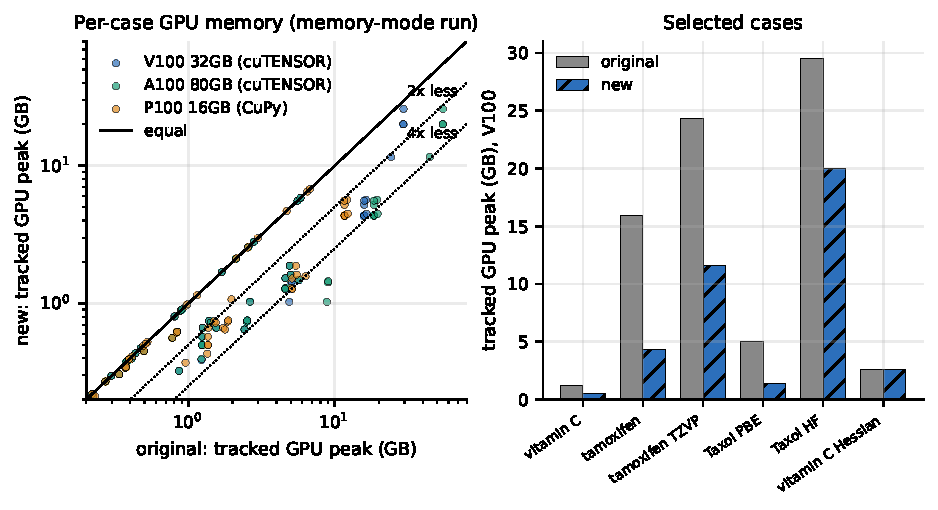
\includegraphics[width=\textwidth]{fig_memory.pdf}
\caption{Tracked GPU memory peak of the new against the original code. Left: every case with an original peak above 0.2~GB (the statistics in the text use 0.3~GB) on three strata (diagonal: equal; dotted: 2$\times$ and 4$\times$ less). Right: selected cases on the V100.}
\label{fig:memory}
\end{figure}

\subsection{Storage tiers}

The fitted integrals can be kept on the GPU, in pinned host memory, or (new code only) in a file read back in bounded blocks. Table~\ref{tab:storage} and Figure~\ref{fig:storage} give time and GPU memory for Taxol (which has a CPU reference and passes the accuracy gate in every tier for the new code) and for valinomycin (1542 basis functions, a capacity observation). Taxol on the V100 takes 59.3 s resident on the GPU, 71.7 s with the integrals in host memory (+21\%) and 254.5 s from disk, while the gradient-phase GPU peak falls to 4.1~GB in every tier (6.6~GB for the A100 disk run, which was made before the final gradient changes); the original code needs 29.6~GB for the gradient even with the integrals in host memory, and 54.9~GB on the A100. On the A100 the host tier costs +31\% (46.4 s against 35.4 s) because the faster card hides less of the transfer. On the 12 and 16~GB P100 cards neither the original code nor the GPU-resident new code can start Taxol with a hybrid functional (the 15.5~GB fitted-integral tensor alone does not fit), but the new code with host memory completes it in 111.5 and 91.5 s using 4.7~GB of GPU memory. Valinomycin does not fit the 32~GB V100 in either code version when resident (31.5~GB tensor); with host memory the original code needs 75.5~GB of GPU memory for its gradient (A100; this peak is card dependent, because the original workspace is sized from the free memory, and is not a minimum) while the new code needs 8.7~GB, so valinomycin runs on both P100 cards (265 s on the 12~GB and 221 s on the 16~GB card). The disk tier is 1.3--6$\times$ slower than host memory, depending on system and card (3--5.4$\times$ for Taxol and valinomycin); its times depend on the shared filesystem (Section~\ref{sec:limits}).

\begin{table}[!htbp]
\centering
\small
\resizebox{\textwidth}{!}{%
\begin{tabular}{lllrrr}
\toprule
system & card & version / tier & time (s) & GPU peak, gradient (GB) & host RSS (GB) \\
\midrule
Taxol (1123 AOs) & V100 32GB & orig. GPU & 59.1 & 29.6 & -- \\
 & V100 32GB & orig. host & 70.8 & 29.6 & 17 \\
 &  & new GPU & 59.3 & 4.1 & 1 \\
 &  & new host & 71.7 & 4.1 & 17 \\
 &  & new disk & 254.5 & 4.1 & 3 \\
 & A100 80GB & orig. GPU & 33.7 & 54.9 & -- \\
 & A100 80GB & orig. host & 43.8 & 54.9 & 17 \\
 &  & new GPU & 35.4 & 4.1 & 1 \\
 &  & new host & 46.4 & 4.1 & 17 \\
 &  & new disk & 215.2$^\dagger$ & 6.6$^\dagger$ & 3 \\
 & P100 16GB & orig. GPU & out of memory & -- & -- \\
 & P100 16GB & orig. host & out of memory & -- & -- \\
 &  & new host & 91.5 & 4.7 & 16 \\
 & P100 12GB & orig. GPU & out of memory & -- & -- \\
 & P100 12GB & orig. host & out of memory & -- & -- \\
 &  & new host & 111.5 & 4.7 & 16 \\
\midrule
valinomycin (1542 AOs) & V100 32GB & orig. GPU & out of memory & -- & -- \\
 & V100 32GB & orig. host & 174.4 & -- & 33 \\
 &  & new GPU & out of memory & -- & -- \\
 &  & new host & 185.0$^\dagger$ & 14.8$^\dagger$ & 33 \\
 &  & new disk & 577.6$^\dagger$ & 14.8$^\dagger$ & 6 \\
 & A100 80GB & orig. GPU & 79.4 & -- & 1 \\
 & A100 80GB & orig. host & 88.2 & 75.5 & 33 \\
 &  & new GPU & 79.1$^\dagger$ & 14.8$^\dagger$ & 1 \\
 &  & new host & 97.2 & 8.7 & 33 \\
 &  & new disk & 524.4$^\dagger$ & 14.8$^\dagger$ & 6 \\
 & P100 16GB & orig. host & out of memory & -- & -- \\
 &  & new host & 220.9 & 8.7 & 32 \\
 & P100 12GB & orig. host & out of memory & -- & -- \\
 &  & new host & 264.9 & 8.7 & 32 \\
\bottomrule
\end{tabular}}
\caption{Storage tiers for the fitted integrals. Taxol has a CPU reference and passes the accuracy gate for the new code in every tier (the original code fails its gradient gate); valinomycin is a capacity observation. The original code has no disk tier. Rows marked $\dagger$ were run before the final gradient-memory fixes (their gradient peaks are 6.6 and 14.8 GB instead of 4.1 and 8.7 GB); all other new-code rows use the final code.}
\label{tab:storage}
\end{table}

\begin{figure}[!htbp]
\centering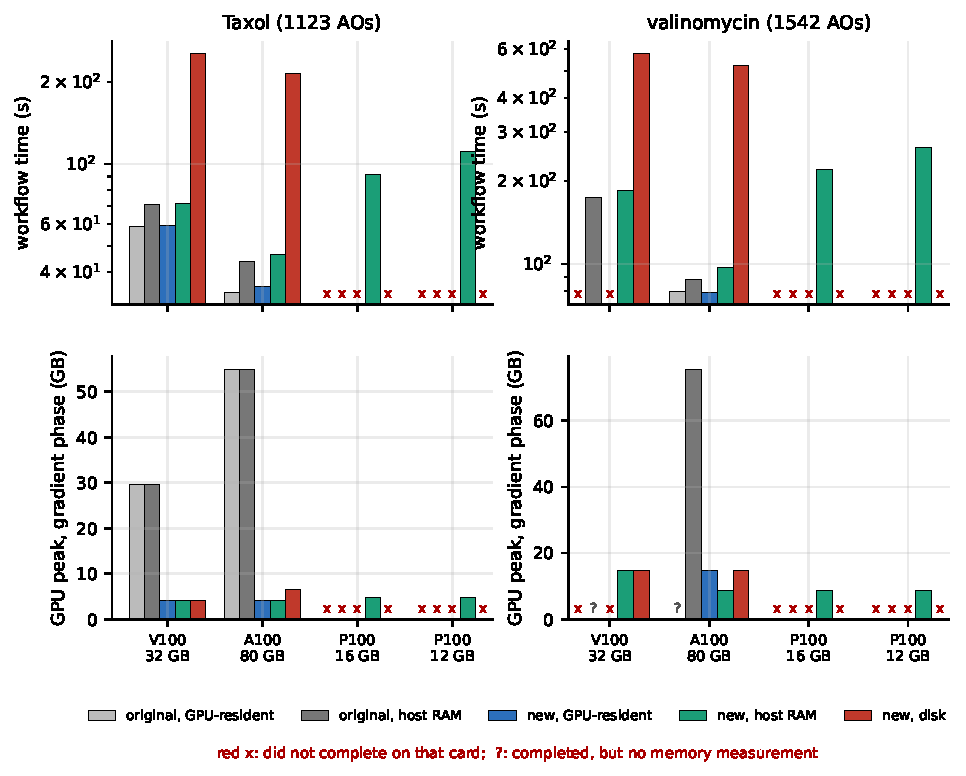
\includegraphics[width=\textwidth]{fig_storage_tiers.pdf}
\caption{Time (top) and gradient-phase GPU memory (bottom) of Taxol (left) and valinomycin (right) by storage tier and card.}
\label{fig:storage}
\end{figure}

\subsection{Capacity ladder}

Table~\ref{tab:capacity} and Figure~\ref{fig:capacity} give the largest system each code version and tier completed with a B3LYP/def2-SVP energy and full-response gradient. The new code completes a cluster of 139 water molecules (\BiggestAtoms{} atoms, \BiggestAOs{} basis functions) on the A100 in 17.9 min with host memory and 45.6 min from disk, against 300 atoms (2400 functions) for the original code; on the 32~GB V100 it reaches a 213-atom glycine chain (2154 functions) against a 76-water cluster of 228 atoms (1824 functions) for the original with host memory (the ladder mixes system families, and each entry is a lower bound at rung granularity), while resident on the GPU both versions stop at Taxol (1123 functions); on the two P100 cards it reaches valinomycin (168 atoms, 1542 functions) against tamoxifen (57 atoms, 537 functions) for the original, so a 12~GB card treats a system roughly three times larger (this P100 comparison mixes the memory and engine effects: the original code with host memory already reaches valinomycin on the 16~GB V100 with cuTENSOR); the 16~GB V100 reaches valinomycin with both versions (the original with host memory). These are capacity observations without a CPU reference.

\begin{table}[!htbp]
\centering
\small
\resizebox{\textwidth}{!}{%
\begin{tabular}{llcrrr}
\toprule
card & version / tier & largest system & atoms & AOs & time (min) \\
\midrule
P100 12GB & orig. GPU & tamoxifen & 57 & 537 & 0.39 \\
 & orig. host & tamoxifen & 57 & 537 & 0.42 \\
 & new GPU & tamoxifen & 57 & 537 & 0.22 \\
 & new host & valinomycin & 168 & 1542 & 4.41 \\
 & new disk & valinomycin & 168 & 1542 & 12.0 \\
\midrule
P100 16GB & orig. GPU & tamoxifen & 57 & 537 & 0.27 \\
 & orig. host & tamoxifen & 57 & 537 & 0.39 \\
 & new GPU & tamoxifen & 57 & 537 & 0.20 \\
 & new host & valinomycin & 168 & 1542 & 3.70 \\
 & new disk & valinomycin & 168 & 1542 & 12.9 \\
\midrule
V100 16GB & orig. GPU & tamoxifen & 57 & 537 & 0.13 \\
 & orig. host & valinomycin & 168 & 1542 & 3.17 \\
 & new GPU & tamoxifen & 57 & 537 & 0.14 \\
 & new host & valinomycin & 168 & 1542 & 3.05 \\
 & new disk & valinomycin & 168 & 1542 & 11.5 \\
\midrule
V100 32GB & orig. GPU & Taxol & 113 & 1123 & 0.94 \\
 & orig. host & (H$_2$O)$_{76}$ & 228 & 1824 & 4.54 \\
 & new GPU & Taxol & 113 & 1123 & 0.97 \\
 & new host & gly30 & 213 & 2154 & 8.99 \\
 & new disk & gly30 & 213 & 2154 & 11.7 \\
\midrule
A100 80GB & orig. GPU & (H$_2$O)$_{100}$ & 300 & 2400 & 4.29 \\
 & orig. host & (H$_2$O)$_{100}$ & 300 & 2400 & 4.58 \\
 & new GPU & gly40 & 283 & 2864 & 9.82 \\
 & new host & (H$_2$O)$_{139}$ & 417 & 3336 & 17.9 \\
 & new disk & (H$_2$O)$_{139}$ & 417 & 3336 & 45.6 \\
\bottomrule
\end{tabular}}
\caption{Largest system completed with B3LYP/def2-SVP energy and full-response gradient. These are capacity observations: no CPU reference exists, so only finite values and convergence are checked.}
\label{tab:capacity}
\end{table}

\begin{figure}[!htbp]
\centering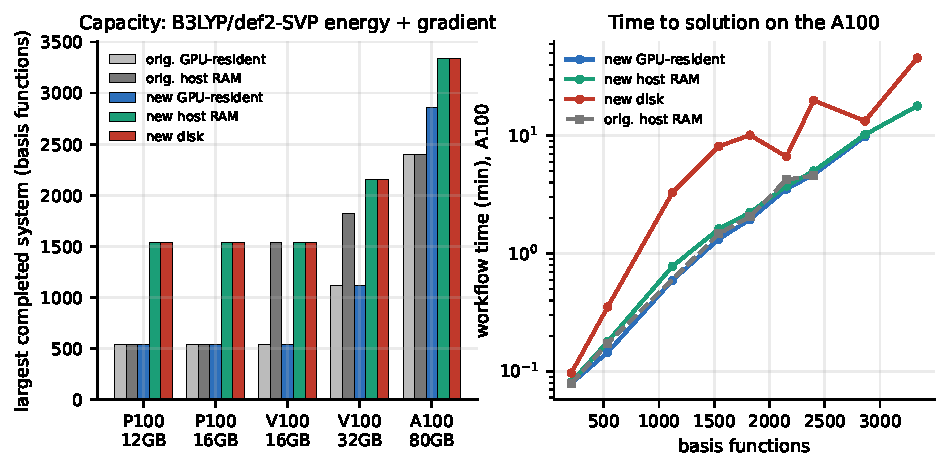
\includegraphics[width=\textwidth]{fig_capacity.pdf}
\caption{Left: largest system completed by card, code version and storage tier. Right: workflow time on the A100 against system size.}
\label{fig:capacity}
\end{figure}

\paragraph{What limits larger systems.} Beyond these rungs the limit is not the fitted-integral tensor but a tensor of $N_\mathrm{aux}N_\mathrm{occ}^2$ elements ($N_\mathrm{aux}$ counted in Cartesian functions) that the analytic gradient holds on the GPU whichever storage tier is used. It is 2.7~GB for Taxol, 6.4~GB for valinomycin, 26.6~GB for the 100-water cluster, 50.1~GB for the 40-residue glycine chain, 71.4~GB for the 139-water cluster, and 97.3~GB for the 50-residue chain, which exceeds the 80~GB of the A100 and ends the ladder there. The storage tiers of the fitted integrals are therefore exhausted at about 3300 basis functions on the largest card; going further requires the gradient to hold this tensor in host memory in blocks, which is not implemented.

\section{Discussion}
\label{sec:discussion}

\paragraph{What the changes buy.} (i) \emph{Memory}: a median of about 2$\times$ (1.8--2.5$\times$ by stratum) and up to 4.8$\times$ (V100) or 8.6$\times$ (A100) less tracked GPU memory, which together with the new disk tier and the host tier lets a 12~GB GPU treat systems of about 1500 basis functions and an 80~GB GPU systems of about 3300. (ii) \emph{Speed on the fallback engine}: 1.2--1.8$\times$ for intermediate-size hybrid-functional jobs, up to 2.4$\times$. (iii) \emph{No loss of accuracy}: the worst qualified errors are the same or smaller than for the original code. The changes do \emph{not} accelerate jobs that already use cuTENSOR, where the new code is on average 0--1\% different from the original and up to 12\% slower for Hartree--Fock and hybrid functionals in mid-size cases, nor jobs that do not call the modified paths directly (TDDFT, MP2, CCSD, properties, periodic; Hessians and optimizations differ by a few percent at most).

\paragraph{Relation to the earlier GB10 study.} The earlier study reported 1.47$\times$ for tamoxifen and 1.95$\times$ for Taxol (Table~\ref{tab:gb10}). Here the same direction appears only without cuTENSOR and with smaller factors; with cuTENSOR it disappears. The GB10 had no cuTENSOR bindings, much lower double-precision throughput and unified memory, so its result describes cards and installations without a working cuTENSOR (for example, hardware without cuTENSOR bindings) rather than datacenter GPUs.

\paragraph{Recommendations.} (1) Keep cuTENSOR as the default engine where available: over the cases where the new code takes at least five seconds, the CuPy engine makes the original code slower than cuTENSOR by a median of 1.12--1.14$\times$ and by up to 2.57$\times$ (tamoxifen B3LYP/def2-TZVP on the A100), while for the new code the median is 1.02--1.06$\times$ and the maximum 1.30$\times$ (this CuPy-over-cuTENSOR ratio is a different quantity from the original/new ratio quoted elsewhere). (2) Treat the new code's value on such systems as memory and capacity, and on fallback-engine systems also speed. (3) The next memory limit is the gradient tensor; offloading it to host memory in auxiliary blocks would extend all tiers. (4) The remaining time is dominated by the exchange build near the measured cuBLAS double-precision rate and, for mid-size systems, by the XC quadrature (73\% of the tamoxifen SCF on the A100), which is where further speed work would have to focus; neither start-up costs (Section~\ref{sec:cold}) nor the SCF cycle count offer large gains.
